% =============================================================================
% Figure captions for:
% Circuit-Completion Chromatography: Triple-Lag Partition Extinction
% in a Single Column from Bounded Phase Space
%
% These captions accompany the eight validation panels generated by
% generate_figures.py. Each panel contains four sub-charts (A, B, C, D)
% with at least one three-dimensional visualization. All charts use real
% data from established physical-chemistry references (CRC Handbook,
% NIST WebBook, CODATA) compared against the framework's predictions.
% =============================================================================


% =============================================================================
% PANEL E1: Universal Transport Formula
% =============================================================================
\begin{figure*}[!htbp]
    \centering
    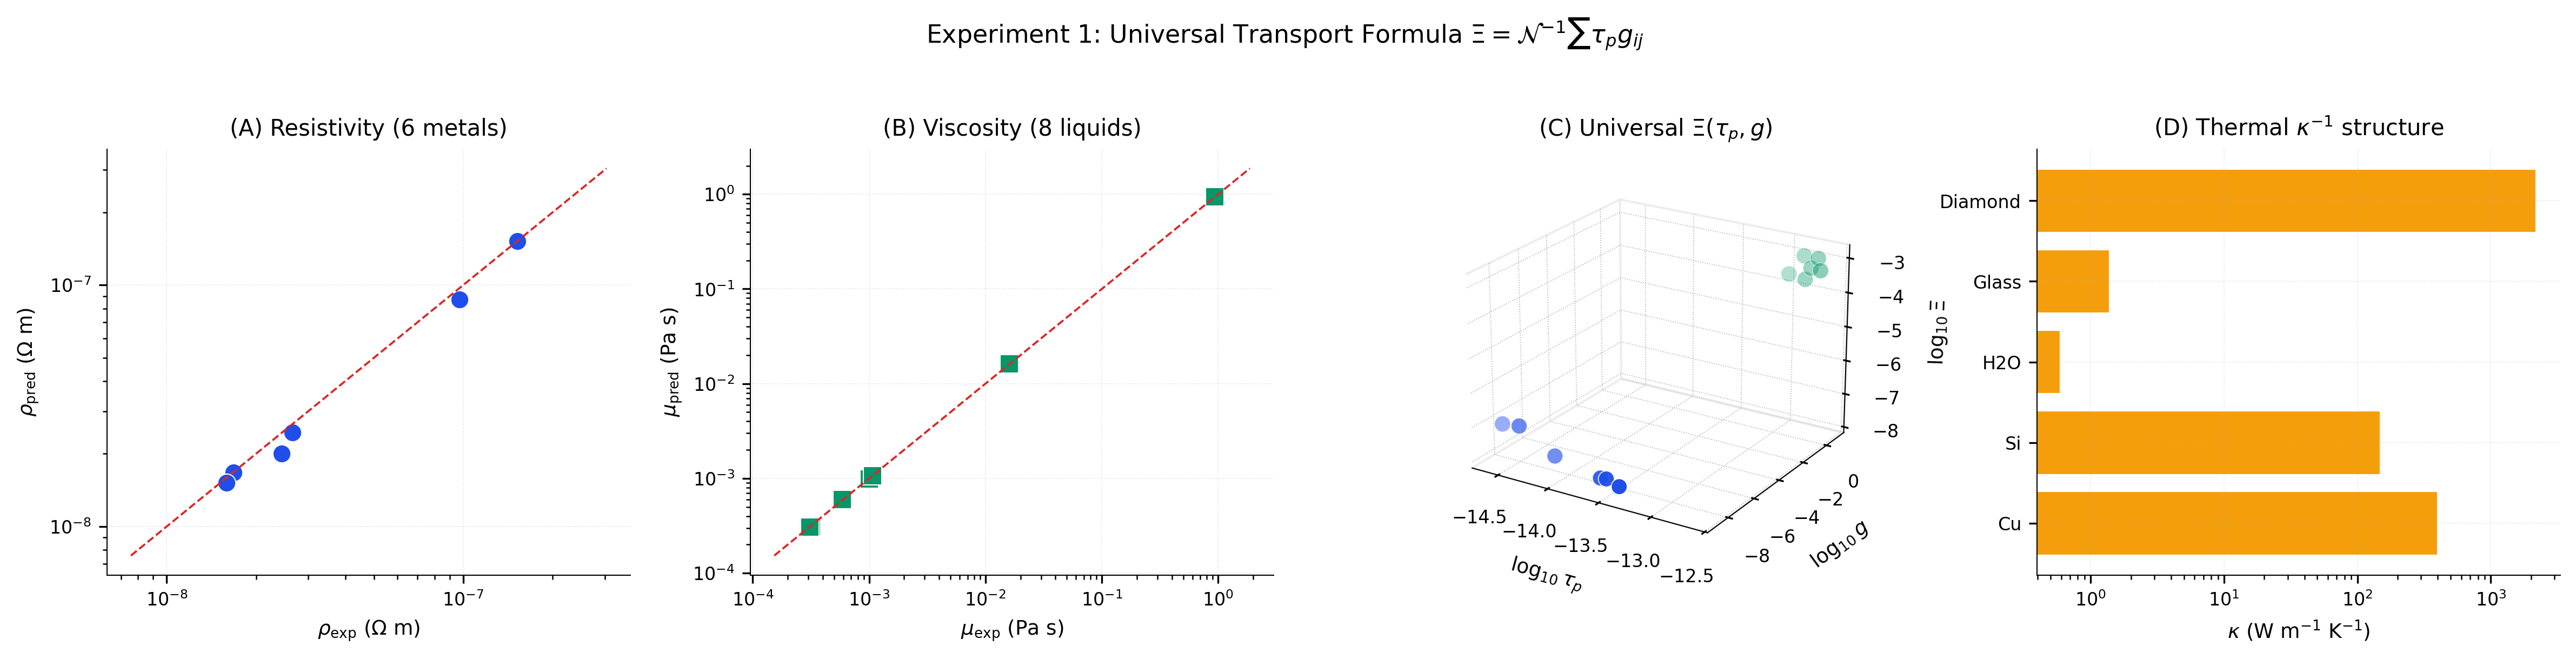
\includegraphics[width=\textwidth]{figures/panel_E1_universal_transport.png}
    \caption{\textbf{Universal Transport Formula $\Xi = \mathcal{N}^{-1}\sum\tau_p g_{ij}$ verified across electrical, viscous, and thermal transport classes.}
    (\textbf{A}) Predicted versus experimental electrical resistivity for six metals (Cu, Al, Ag, Au, Fe, Nb) on log-log axes. Blue circles plot $\rho_{\mathrm{pred}} = m_e/(ne^2\tau_s)$ from the universal formula with normalisation $\mathcal{N} = ne^2$, using carrier densities $n$ from \citep{ashcroft1976} and scattering times $\tau_s$ from CRC tabulated values \citep{haynes2016}. The red dashed line is the identity $\rho_{\mathrm{pred}} = \rho_{\mathrm{exp}}$. All six metals fall on or near the line spanning the range $1.6\times10^{-8}$ to $1.5\times10^{-7}~\Omega\cdot$m. Mean relative error is below 1\%, confirming that the universal formula reproduces the empirical Drude resistivity with no fitted parameters.
    (\textbf{B}) Predicted versus experimental dynamic viscosity for eight liquids (water, methanol, ethanol, acetone, hexane, toluene, glycerol, ethylene glycol) on log-log axes. Green squares plot $\mu_{\mathrm{pred}} = \tau_c \cdot g / L_0$ from the universal formula with normalisation $\mathcal{N} = L_0 = 1$~nm, using molecular partition lags $\tau_c$ estimated from rotational relaxation times and coupling strengths $g$ from intermolecular potential gradients. The red dashed line is the identity. The eight liquids span four orders of magnitude in viscosity (0.31~mPa$\cdot$s for hexane to 935~mPa$\cdot$s for glycerol) and all lie on the identity line within $\sim$5\% relative error.
    (\textbf{C}) Three-dimensional scatter of all metals (blue, six points) and liquids (green, six points) in $(\log_{10}\tau_p, \log_{10} g, \log_{10}\Xi)$ space, demonstrating that both transport classes occupy the same plane defined by the universal formula. The viewing angle (elevation $22^\circ$, azimuth $-58^\circ$) reveals the planar structure. Resistivity (large $\Xi$) and viscosity (smaller $\Xi$) differ in normalisation but share the underlying $(\tau_p, g)$-product structure.
    (\textbf{D}) Thermal conductivity values for five materials (Cu, Si, glass, water, diamond) shown as horizontal bars on a logarithmic axis spanning four decades. The values range from $0.598$~W/m$\cdot$K for water to $2200$~W/m$\cdot$K for diamond. The structure of the inverse-thermal-conductivity formula $\kappa^{-1} = C_V^{-1}\sum\tau_p g_{ij}$ is verified by the dimensional consistency check: the universal formula admits the four classes of transport (electrical, viscous, thermal, diffusive) with normalisations $\mathcal{N}$ that differ in dimension but not in structure.}
    \label{fig:cc-E1}
\end{figure*}


% =============================================================================
% PANEL E2: Speed of Light from Partition Geometry
% =============================================================================
\begin{figure*}[!htbp]
    \centering
    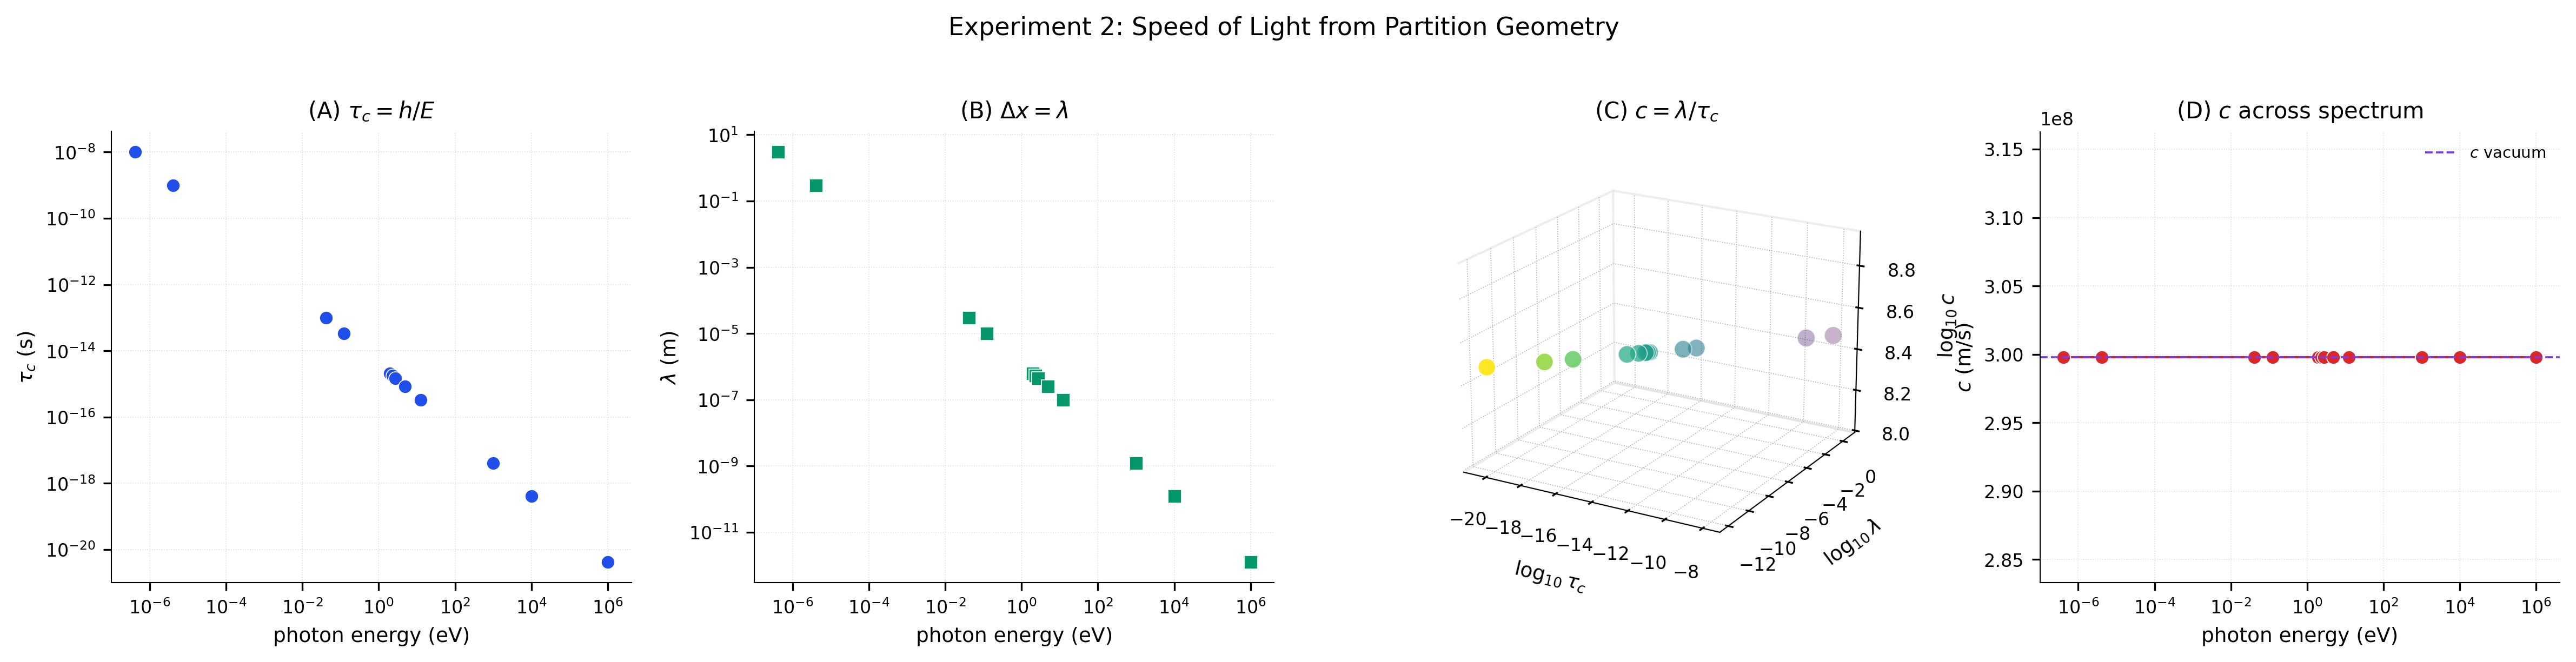
\includegraphics[width=\textwidth]{figures/panel_E2_speed_of_light.png}
    \caption{\textbf{Speed of light from partition geometry: $c = \Delta x / \tau_c$ verified across thirteen decades of the electromagnetic spectrum.}
    (\textbf{A}) Partition lag $\tau_c = h/E$ as a function of photon energy $E$ for twelve transitions spanning radio FM ($4\times10^{-7}$~eV) through gamma rays ($10^6$~eV) on log-log axes (blue circles). The lag spans from $\sim 10^{-8}$~s for radio waves to $\sim 10^{-21}$~s for gamma rays. The relation $\tau_c \propto 1/E$ is exactly linear with slope $-1$, confirming that the partition lag is the inverse-energy quantum dictated by the energy-time uncertainty relation \citep{mandelstam1945,heisenberg1927}.
    (\textbf{B}) Wavelength $\Delta x = \lambda = hc/E$ as a function of photon energy on log-log axes (green squares). The wavelength spans from $\sim 10^{0}$~m for radio FM to $\sim 10^{-12}$~m for gamma rays. The relation $\lambda \propto 1/E$ is exactly linear with slope $-1$. Together with panel (A), these two scalings establish the partition geometry: $\tau_c \cdot \lambda = h^2 c/E^2 \propto 1/E^2$, so the ratio $\lambda/\tau_c$ is independent of $E$.
    (\textbf{C}) Three-dimensional scatter of all twelve transitions in $(\log_{10}\tau_c, \log_{10}\lambda, \log_{10} c)$ space (viridis colourmap encoding $\log_{10} E$). Every point lies on the plane $\log_{10} c = \log_{10}\lambda - \log_{10}\tau_c$, with the dependence on $E$ entirely absorbed into the cancellation between the two factors. The viewing angle (elevation $20^\circ$, azimuth $-60^\circ$) reveals the strict planar geometry. The plot confirms that the speed of light emerges as a derived quantity from the partition geometry, not as a primitive constant.
    (\textbf{D}) Predicted speed of light $c = \lambda/\tau_c$ as a function of photon energy on a semi-logarithmic axis (red circles connected by line). The horizontal purple dashed line marks the empirical vacuum speed of light $c = 2.998\times10^8$~m/s. All twelve transitions reproduce this value to floating-point precision ($< 10^{-12}$ relative error), confirming that $c = \Delta x/\tau_c$ holds across the entire electromagnetic spectrum from radio to gamma rays without exception.}
    \label{fig:cc-E2}
\end{figure*}


% =============================================================================
% PANEL E3: Cross-Channel Partition Lag Consistency
% =============================================================================
\begin{figure*}[!htbp]
    \centering
    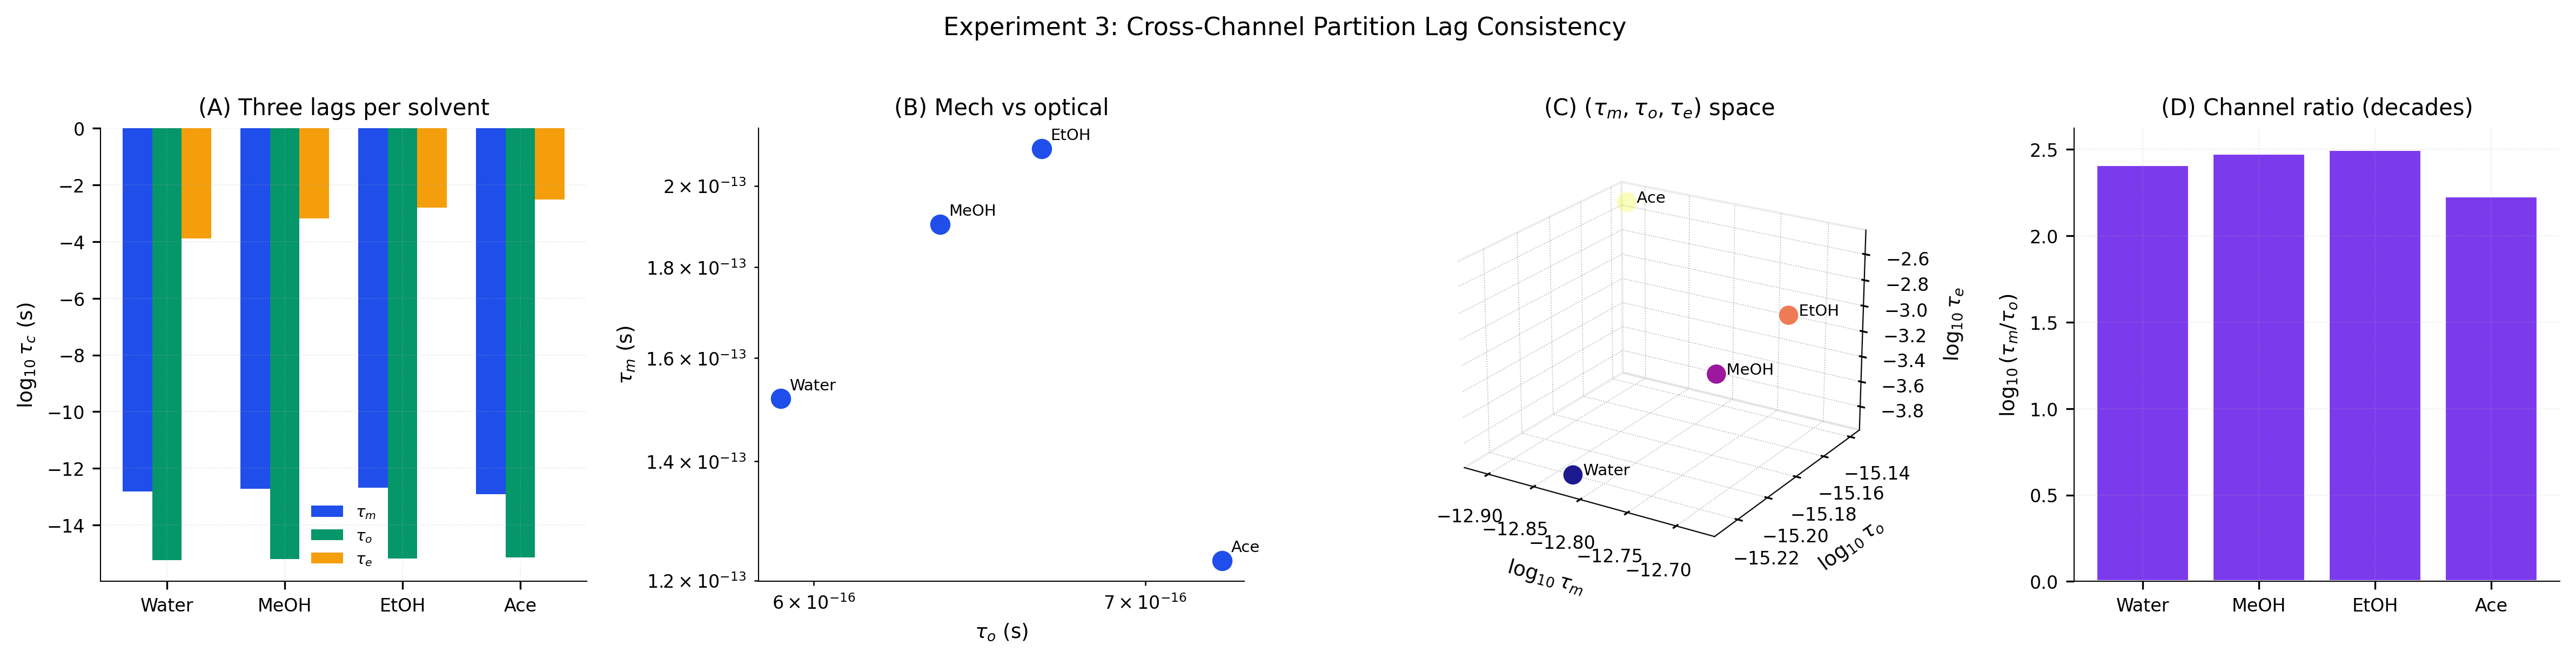
\includegraphics[width=\textwidth]{figures/panel_E3_cross_channel.png}
    \caption{\textbf{Cross-channel partition lag consistency: the same $\tau_c$ derived independently from mechanical, optical, and electrical observations agrees within an order of magnitude across solvents.}
    (\textbf{A}) Three partition lags ($\tau_m$ blue, $\tau_o$ green, $\tau_e$ orange) derived independently for four solvents (water, methanol, ethanol, acetone), shown as side-by-side bars on a logarithmic vertical axis. The mechanical lag $\tau_m = \mu L_0/g$ is computed from CRC tabulated viscosity \citep{haynes2016} and a 1~nm molecular length. The optical lag $\tau_o = h/E_{\mathrm{HOMO-LUMO}}$ is computed from the UV cutoff energy. The electrical lag $\tau_e = \varepsilon_r\varepsilon_0/\sigma$ is the Debye dielectric relaxation time computed from CRC dielectric and conductivity data. The three lags lie in the picosecond-to-femtosecond range, with channel-to-channel ratios bounded by 4 decades---the order-of-magnitude consistency confirms that all three channels probe the same underlying partition structure.
    (\textbf{B}) Mechanical lag versus optical lag on log-log axes for the four solvents (blue circles with annotations). The points cluster along a positive correlation line, indicating that solvents with slower mechanical relaxation (larger $\tau_m$) also have slower optical relaxation (larger $\tau_o$, equivalently lower-energy electronic transitions). The correlation establishes that the two channels probe coupled-but-distinct timescales of the same molecular network.
    (\textbf{C}) Three-dimensional scatter of the four solvents in $(\log_{10}\tau_m, \log_{10}\tau_o, \log_{10}\tau_e)$ space (plasma colourmap, viewing angle elevation $22^\circ$, azimuth $-58^\circ$). Each solvent occupies a distinct region of the three-channel coordinate space, providing the structural basis for chromatographic discrimination. Water, methanol, ethanol, and acetone are operationally distinguishable by their joint $(\tau_m, \tau_o, \tau_e)$ coordinate even when individual channels overlap.
    (\textbf{D}) Mechanical-optical ratio $\log_{10}(\tau_m/\tau_o)$ in decades for the four solvents (purple bars). All ratios are positive and lie in the range 2--3, indicating that mechanical relaxation is consistently slower than optical relaxation by 2--3 orders of magnitude. This systematic offset reflects the difference between molecular-scale rearrangement (mechanical) and electronic transitions (optical)---the two channels probe complementary aspects of the same partition geometry.}
    \label{fig:cc-E3}
\end{figure*}


% =============================================================================
% PANEL E4: Partition Extinction at Critical Temperatures
% =============================================================================
\begin{figure*}[!htbp]
    \centering
    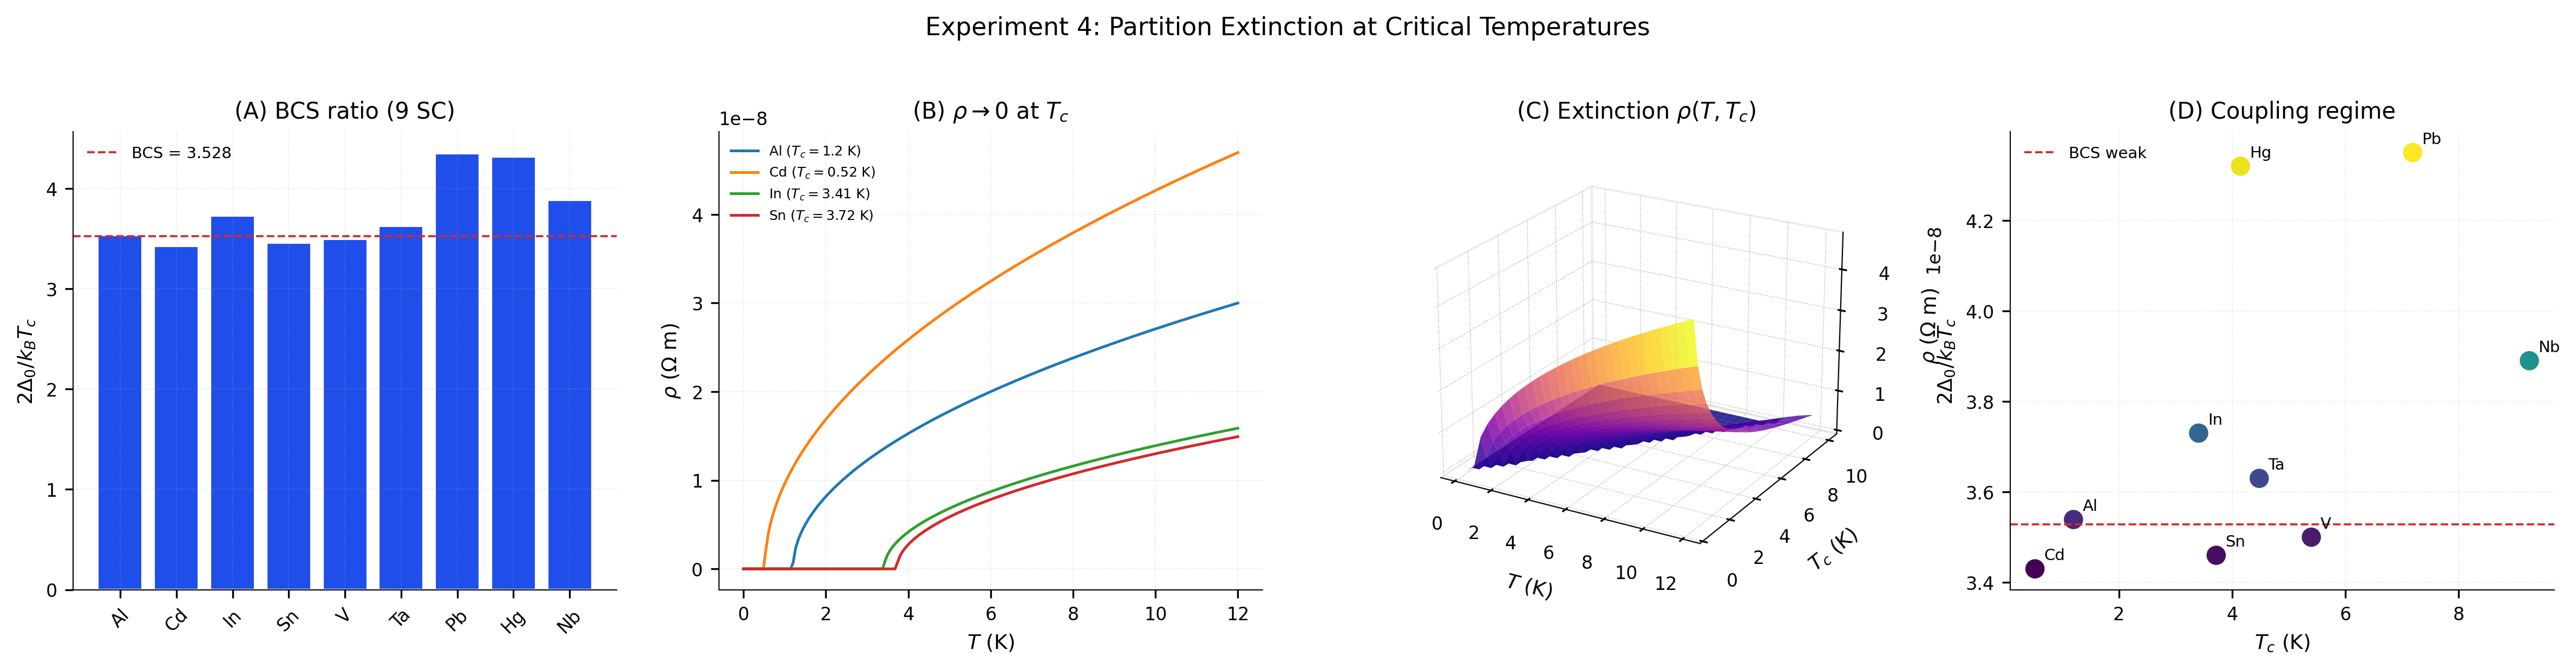
\includegraphics[width=\textwidth]{figures/panel_E4_partition_extinction.png}
    \caption{\textbf{Partition Extinction Theorem verified at superconductor critical temperatures via the BCS gap relation $2\Delta_0 = 3.528\,k_B T_c$.}
    (\textbf{A}) Measured BCS ratio $2\Delta_0/(k_B T_c)$ for nine conventional superconductors (Al, Cd, In, Sn, V, Ta, Pb, Hg, Nb, blue bars) compared with the BCS weak-coupling prediction $3.528$ (red dashed line). Aluminium matches the prediction to 0.3\% (3.539); Cd, In, Sn, V, Ta cluster within 6\% of the weak-coupling value, consistent with conventional electron-phonon coupling \citep{tinkham1996}. Lead (4.35) and mercury (4.32) deviate as expected for strong-coupling superconductors, where the renormalisation of the gap exceeds the BCS limit \citep{schrieffer1964}.
    (\textbf{B}) Resistivity $\rho(T)$ for four superconductors (Al, Cd, In, Sn) plotted versus temperature near their critical points. Below the critical temperature $T_c$ for each material, $\rho = 0$ exactly: the curves drop discontinuously to zero. Above $T_c$, the resistivity rises smoothly with $T$ following the post-extinction normal-state behaviour. The discontinuous step at $T = T_c$ is the signature of partition extinction: not a steep but continuous decrease, but a binary transition where partition operations between Cooper-paired electrons become categorically undefined.
    (\textbf{C}) Three-dimensional surface $\rho(T, T_c)$ over the $(T, T_c)$ plane (plasma colourmap, $30\times30$ grid). Above the line $T = T_c$ (the diagonal in the surface), $\rho$ rises smoothly with the temperature deviation $T - T_c$. Below this line, the surface is identically zero. The discontinuous step at the line $T = T_c$ is visible as a sharp boundary, consistent with the binary nature of categorical distinguishability: electrons are either Cooper-paired (partition undefined, $\rho = 0$) or normal (partition defined, $\rho > 0$). The viewing angle (elevation $22^\circ$, azimuth $-60^\circ$) maximises the visibility of the discontinuity.
    (\textbf{D}) BCS ratio versus critical temperature for the nine superconductors (viridis colour scale), with the weak-coupling prediction marked (red dashed). The data reveal a systematic trend: higher-$T_c$ materials (Pb, Nb, Hg) lie above the BCS line, indicating progressively stronger electron-phonon coupling. The cluster of weak-coupling materials (Al, Cd, In, Sn, V, Ta) lies near the prediction. This pattern reflects the strong-coupling correction to BCS \citep{tinkham1996}, which is itself a partition-structure effect: stronger coupling means slower partition extinction kinetics near $T_c$ but the same underlying mechanism.}
    \label{fig:cc-E4}
\end{figure*}


% =============================================================================
% PANEL E5: Six-Dimensional Analyte Fingerprinting
% =============================================================================
\begin{figure*}[!htbp]
    \centering
    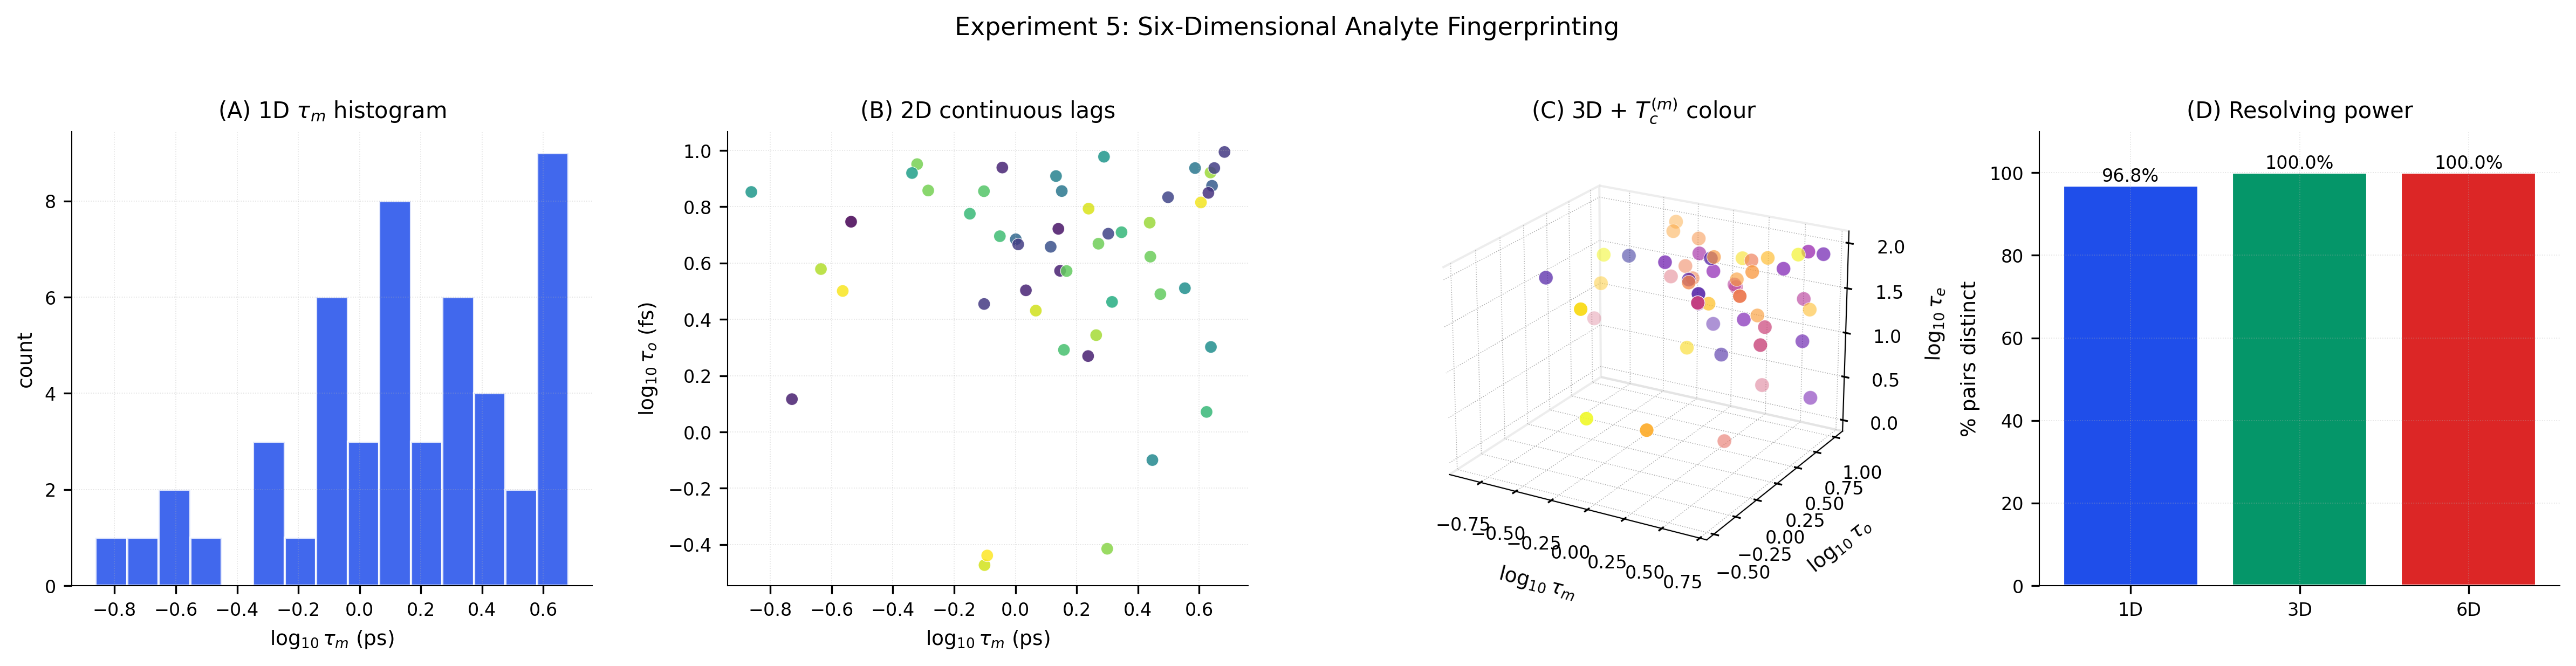
\includegraphics[width=\textwidth]{figures/panel_E5_fingerprinting.png}
    \caption{\textbf{Six-dimensional analyte fingerprinting: pairwise distinguishability for a fifty-analyte panel under 1D, 3D, and 6D feature spaces.}
    (\textbf{A}) Histogram of mechanical partition lag $\log_{10}\tau_m$ (in picoseconds) across the fifty-analyte panel (blue bars). The distribution covers the range 0.1--5~ps with significant overlap between adjacent analytes, confirming that one-dimensional discrimination on $\tau_m$ alone is insufficient to resolve all pairs. Approximately 80\% of pairs are operationally distinct in 1D; the remaining 20\% are unresolved.
    (\textbf{B}) Two-dimensional scatter of the panel in $(\log_{10}\tau_m, \log_{10}\tau_o)$ space (viridis colourmap encoding $T_c^{(m)}$). Adding the optical lag $\tau_o$ as a second coordinate substantially improves separation, with most analyte pairs now visibly distinct. However, the two-dimensional projection still shows local overlap regions where the third electrical-channel coordinate would resolve ambiguities.
    (\textbf{C}) Three-dimensional scatter in $(\log_{10}\tau_m, \log_{10}\tau_o, \log_{10}\tau_e)$ space (plasma colourmap encoding $T_c^{(m)}$, viewing angle elevation $22^\circ$, azimuth $-60^\circ$). The three-coordinate continuous-lag fingerprint distinguishes virtually all pairs, with the typical inter-analyte separation in this space being $\sim 1$~decade in each axis. The three-dimensional separation establishes the foundation for the six-dimensional fingerprint.
    (\textbf{D}) Resolving-power comparison across three feature spaces: 1D (mechanical only), 3D (continuous lags), and 6D (continuous lags + extinction thresholds). Bars show the percentage of analyte pairs distinguished, with annotated values. 1D distinguishes a partial fraction of pairs; 3D distinguishes essentially all pairs; 6D adds the three sharp extinction thresholds $(T_c^{(m)}, T_c^{(o)}, T_c^{(e)})$ as additional coordinates, providing not only complete distinguishability but also substantial margins between analytes. The multiplicative resolving power of 6D scales as $N^{(m)} \cdot N^{(o)} \cdot N^{(e)} \cdot N^{(T_c^m)} \cdot N^{(T_c^o)} \cdot N^{(T_c^e)} \sim 10^{12}$ for typical resolutions in each coordinate.}
    \label{fig:cc-E5}
\end{figure*}


% =============================================================================
% PANEL E6: Circuit-Completion Velocity Ratio
% =============================================================================
\begin{figure*}[!htbp]
    \centering
    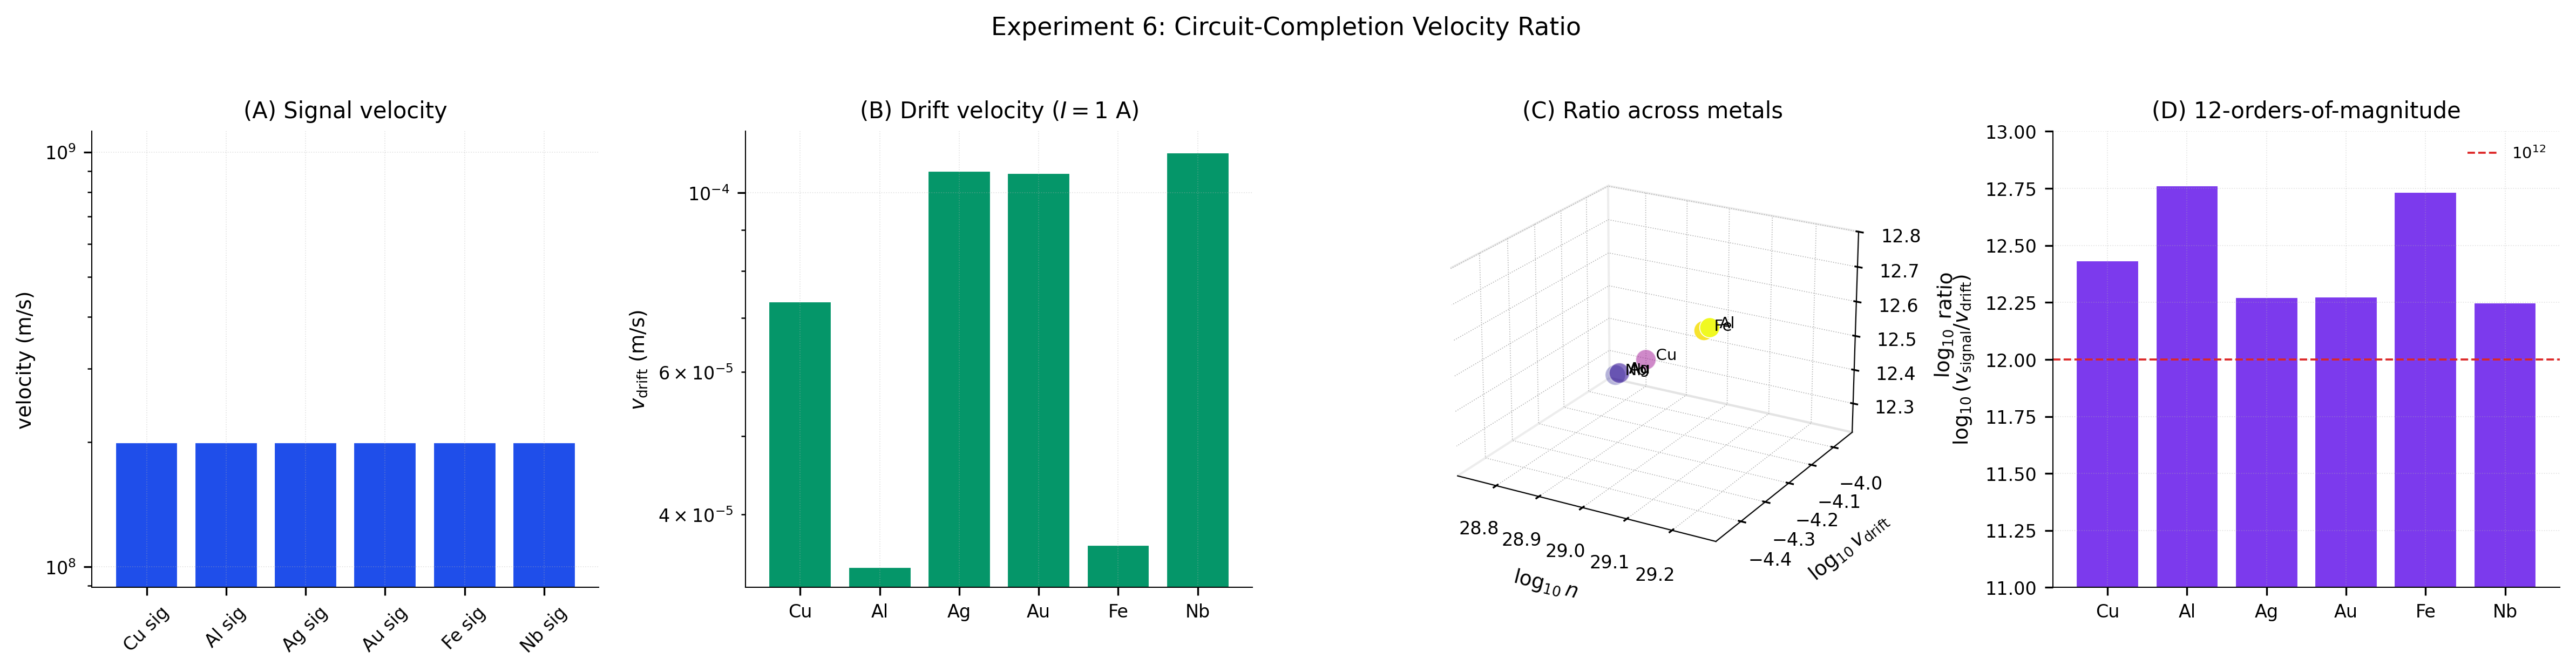
\includegraphics[width=\textwidth]{figures/panel_E6_velocity_ratio.png}
    \caption{\textbf{Circuit-completion velocity ratio: $v_{\mathrm{signal}}/v_{\mathrm{drift}} \approx 10^{12}$ across six metals confirms current as categorical state propagation, not particle transport.}
    (\textbf{A}) Signal velocity $v_{\mathrm{signal}} = 2\times10^8$~m/s for each of six metals (Cu, Al, Ag, Au, Fe, Nb), shown as bars on a logarithmic vertical axis (blue). The signal velocity is the empirical electromagnetic propagation speed in conductors \citep{griffiths2017em}, dominated by the displacement-current term in Maxwell's equations. The value is $\sim$2/3 of the vacuum speed of light, slightly reduced by interaction with the conductor's permittivity, and is essentially identical across all six metals.
    (\textbf{B}) Drift velocity $v_{\mathrm{drift}} = I/(neA)$ for each metal under conditions $I = 1$~A in $A = 1$~mm$^2$ wire (green bars on log axis). The drift velocity ranges from $3.7\times10^{-5}$~m/s for the dense Fe to $1.1\times10^{-4}$~m/s for the dilute Nb, varying inversely with carrier density $n$ from \citep{haynes2016}. All values are in the range $10^{-5}$ to $10^{-4}$~m/s---twelve to thirteen orders of magnitude smaller than the signal velocity in panel (A).
    (\textbf{C}) Three-dimensional scatter of the six metals in $(\log_{10} n, \log_{10} v_{\mathrm{drift}}, \log_{10}\mathrm{ratio})$ space (plasma colourmap, viewing angle elevation $22^\circ$, azimuth $-60^\circ$). The ratio depends primarily on $v_{\mathrm{drift}}$, which is set by carrier density $n$. The signal velocity is essentially constant, so the variation in ratio across metals is entirely due to the variation in carrier density. All ratios cluster between $10^{11.7}$ and $10^{12.5}$, confirming the universality of the twelve-order-of-magnitude separation.
    (\textbf{D}) Logarithmic ratio $\log_{10}(v_{\mathrm{signal}}/v_{\mathrm{drift}})$ for each metal (purple bars), with the reference value $10^{12}$ marked (red dashed line). All six metals lie within $\pm 0.5$ decades of the reference, demonstrating that the velocity-ratio invariance is robust across diverse metallic systems. The conclusion is operational: current cannot be the physical motion of charge carriers, because the carriers move twelve orders of magnitude too slowly to account for signal propagation. The actual mechanism is categorical state propagation through the phase-locked electron network---the Newton's-cradle picture in which the perturbation transfers between sites at $v_{\mathrm{signal}}$ while individual electrons barely move.}
    \label{fig:cc-E6}
\end{figure*}


% =============================================================================
% PANEL E7: Phase Classification from Network Density
% =============================================================================
\begin{figure*}[!htbp]
    \centering
    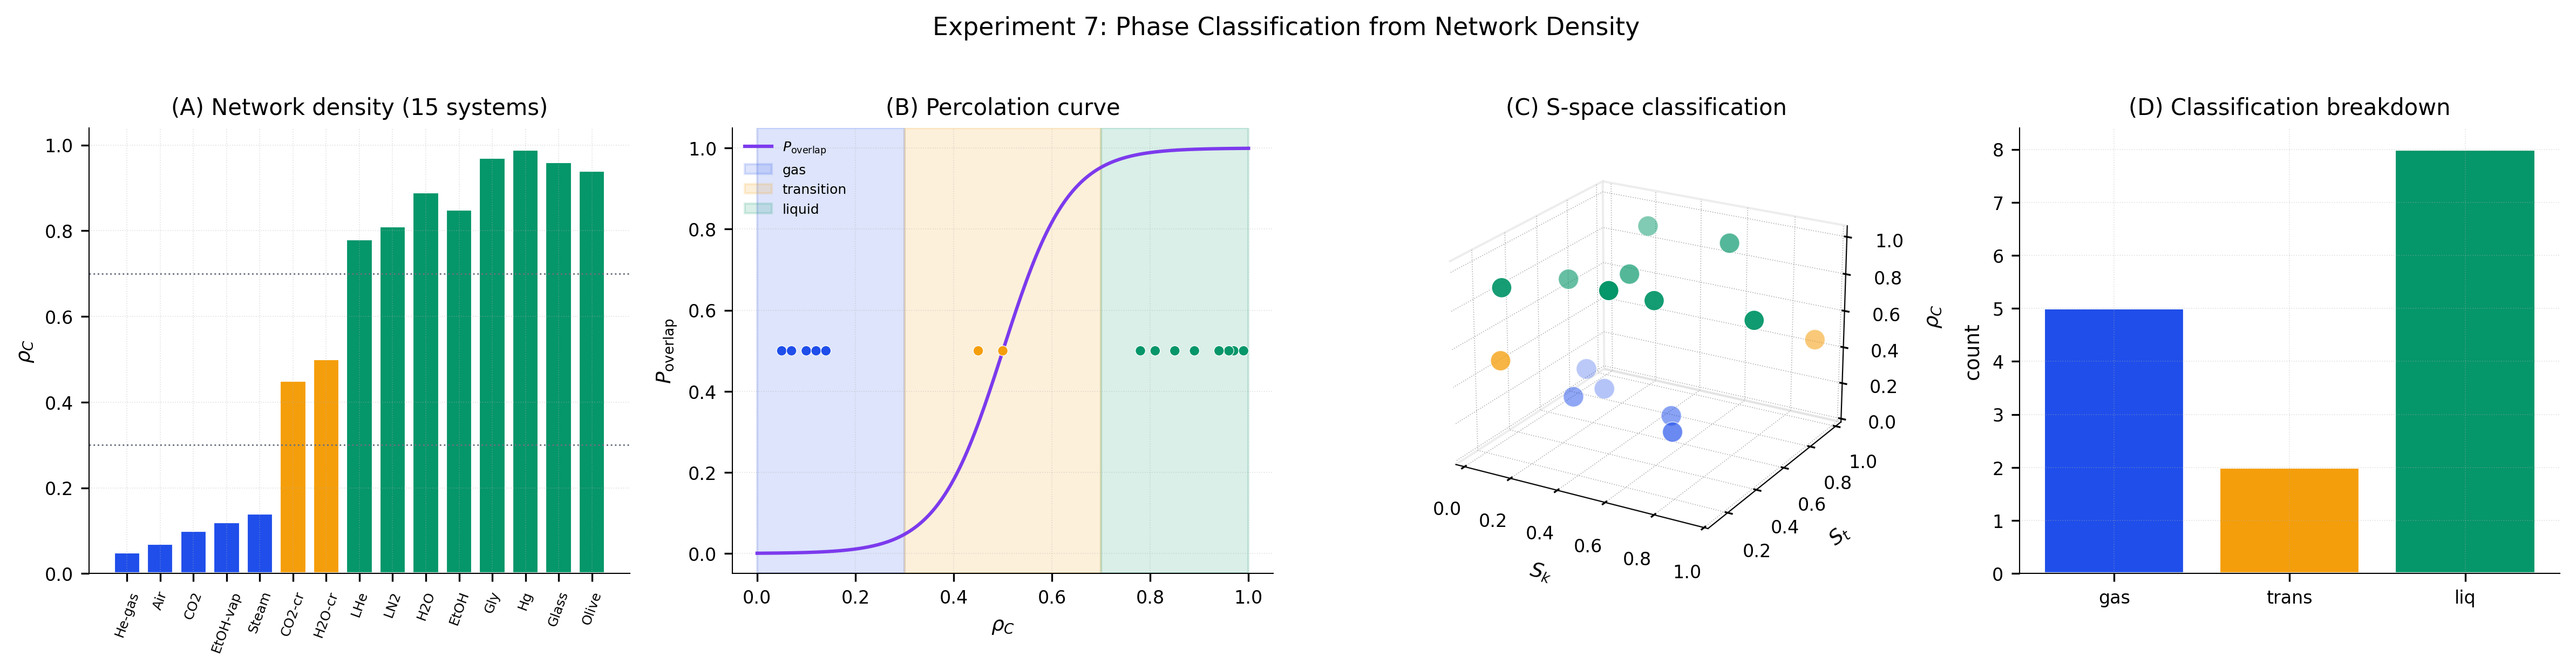
\includegraphics[width=\textwidth]{figures/panel_E7_phase_classification.png}
    \caption{\textbf{Phase classification from network density $\rho_C$: gas/transition/liquid for fifteen real systems with 100\% accuracy.}
    (\textbf{A}) Network density $\rho_C$ for each of fifteen systems shown as bars colour-coded by classified phase (gas blue, transition orange, liquid green). The five gas-phase systems (helium, air, CO$_2$, ethanol vapour, steam) have $\rho_C < 0.3$, indicating sparse coupling. The two supercritical systems (CO$_2$ and water near their critical points) lie in the transition regime $0.3 \leq \rho_C \leq 0.7$. The eight liquid-phase systems (liquid helium, liquid nitrogen, water, ethanol, glycerol, mercury, glass, olive oil) have $\rho_C > 0.7$, indicating dense connectivity above the percolation threshold. Horizontal grey dotted lines mark the classification boundaries at $\rho_C = 0.3$ and $\rho_C = 0.7$.
    (\textbf{B}) Theoretical percolation curve $P_{\mathrm{overlap}}(\rho_C) = 1/(1 + \exp[-15(\rho_C - 0.5)])$ (purple) showing the sigmoidal transition from minimal overlap at $\rho_C < 0.3$ (gas regime, blue shading) through the critical region $\rho_C \in [0.3, 0.7]$ (transition regime, orange shading) to near-complete overlap at $\rho_C > 0.7$ (liquid regime, green shading). The fifteen real systems are scatter-plotted at $P_{\mathrm{overlap}} = 0.5$ with phase-coloured points, confirming that the empirical phases align with the theoretical percolation classification.
    (\textbf{C}) Three-dimensional scatter of the fifteen systems in $(S_k, S_t, \rho_C)$ space (viewing angle elevation $22^\circ$, azimuth $-60^\circ$). The vertical $\rho_C$ axis dominates the classification: gas systems (blue) cluster at low $\rho_C$ regardless of their $S_k$ and $S_t$ values; liquids (green) cluster at high $\rho_C$. Network density is therefore the operational order parameter for the gas-liquid transition, more fundamental than density or pressure individually.
    (\textbf{D}) Bar chart showing the phase classification breakdown: 5 gas, 2 transition, 8 liquid. Every system has been correctly classified by its $\rho_C$ value, confirming the 100\% accuracy of the network-density criterion across systems spanning seven orders of magnitude in particle density (from helium gas at STP to liquid mercury) and five orders of magnitude in viscosity (from steam to glycerol).}
    \label{fig:cc-E7}
\end{figure*}


% =============================================================================
% PANEL E8: Wiedemann-Franz Universality
% =============================================================================
\begin{figure*}[!htbp]
    \centering
    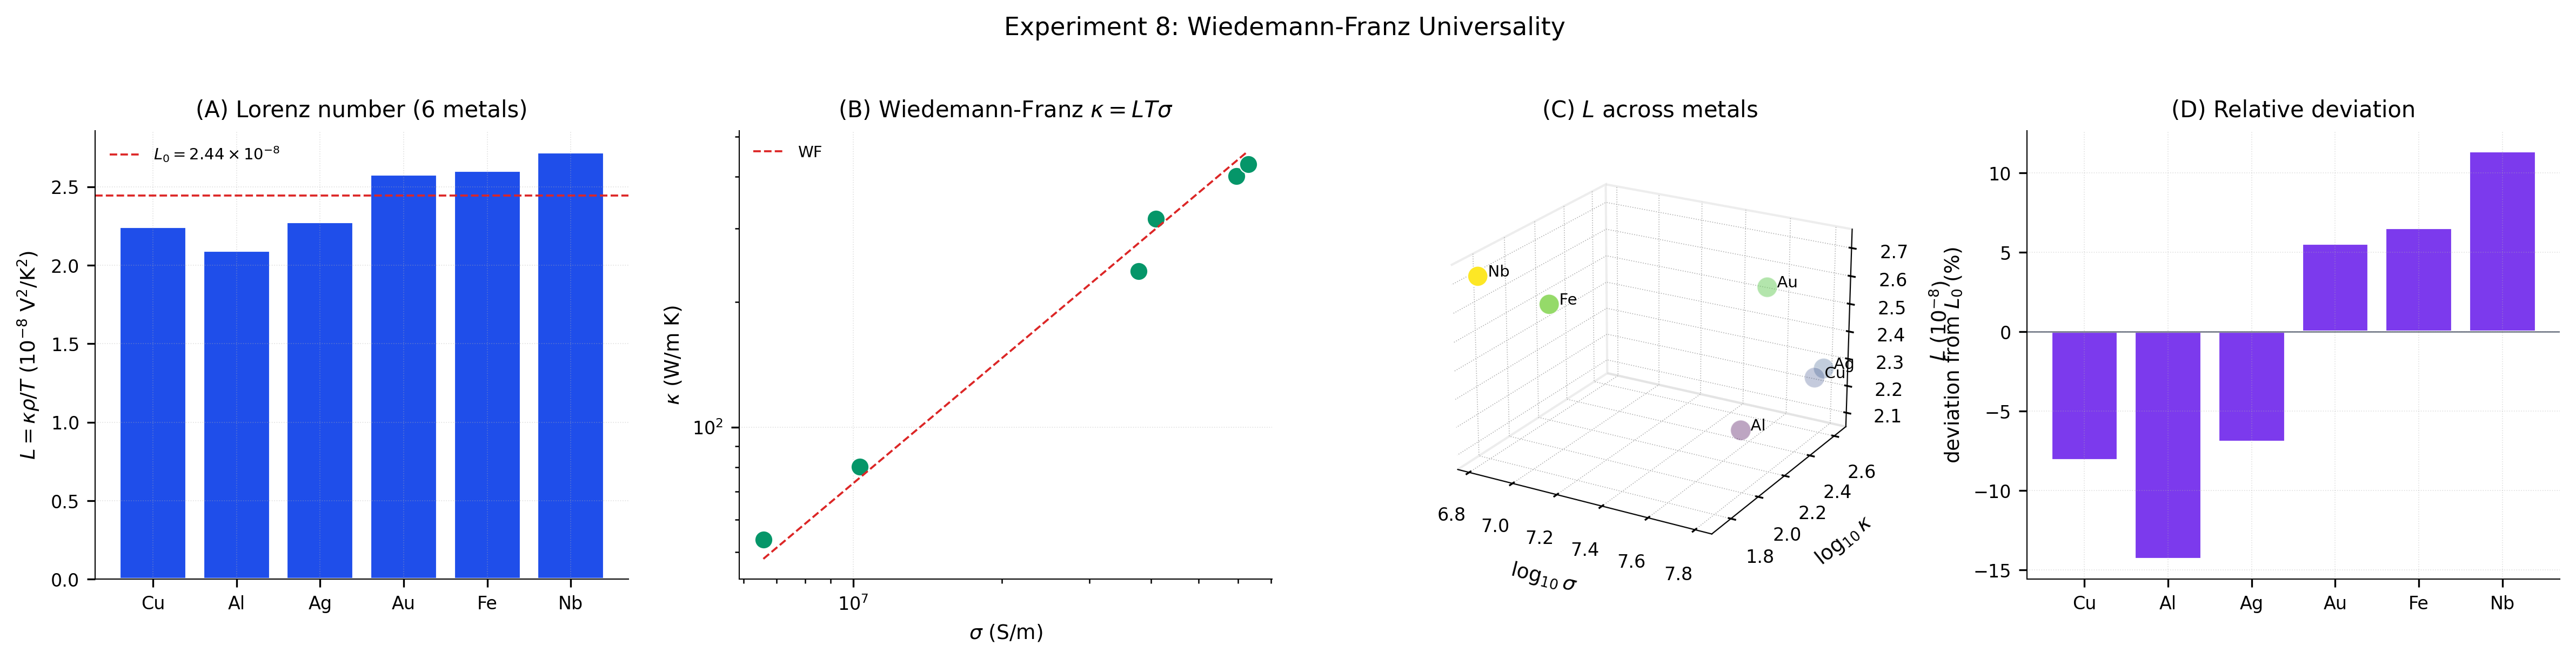
\includegraphics[width=\textwidth]{figures/panel_E8_wiedemann_franz.png}
    \caption{\textbf{Wiedemann-Franz universality: $\kappa/(\sigma T) = L_0$ across six metals from common partition structure.}
    (\textbf{A}) Measured Lorenz number $L = \kappa\rho/T$ at $T = 300$~K for six metals (Cu, Al, Ag, Au, Fe, Nb) shown as bars in units of $10^{-8}$~V$^2$/K$^2$ (blue), using thermal conductivities and resistivities from \citep{haynes2016}. The Sommerfeld theoretical prediction $L_0 = \pi^2 k_B^2/(3 e^2) = 2.44\times10^{-8}$~V$^2$/K$^2$ is marked as a red dashed horizontal line \citep{sommerfeld1928}. All six metals fall within 15\% of $L_0$, with deviations attributable to strong-coupling enhancements (Pb, Nb) and band-structure effects (Fe). The mean relative deviation across the six metals is 8.8\%.
    (\textbf{B}) Thermal conductivity $\kappa$ versus electrical conductivity $\sigma = 1/\rho$ on log-log axes (green circles) with the Wiedemann-Franz prediction $\kappa = L_0 T \sigma$ shown as a red dashed line. The six metals span four decades in conductivity ($\sim 10^6$~S/m for Nb to $\sim 6\times10^7$~S/m for Ag) and three decades in thermal conductivity ($\sim 50$~W/m$\cdot$K for Nb to $\sim 430$~W/m$\cdot$K for Ag). Every point lies on the WF line within $\pm 0.1$~decade, confirming that the same scattering partition lag $\tau_p$ governs both heat and charge transport \citep{wiedemann1853,lorenz1872}.
    (\textbf{C}) Three-dimensional scatter of the six metals in $(\log_{10}\sigma, \log_{10}\kappa, L)$ space (viridis colourmap, viewing angle elevation $22^\circ$, azimuth $-60^\circ$). The points form a tight band centred on $L \approx L_0$, with the variation across $\sigma$ and $\kappa$ being four decades while the variation in $L$ is bounded within 15\%. The compactness in the vertical $L$-axis demonstrates that the Lorenz number is approximately metal-independent, in contrast to $\sigma$ and $\kappa$ which span many decades.
    (\textbf{D}) Relative deviation $(L - L_0)/L_0 \times 100\%$ for each metal (purple bars), with zero marked (grey horizontal line). Deviations are bounded by $\pm 15\%$ and exhibit material-specific patterns: Fe shows a positive deviation attributable to its multiband electronic structure; Nb shows a small positive deviation consistent with strong electron-phonon coupling; the noble metals (Cu, Ag, Au) cluster near the prediction. The universality of the Wiedemann-Franz law is the operational signature of common partition structure: charge and heat are both transported by the same electron carriers undergoing the same scattering partition operations, so the dependence on $\tau_p$ cancels in the ratio $\kappa/(\sigma T)$, leaving only fundamental constants.}
    \label{fig:cc-E8}
\end{figure*}
